\documentclass{article}
\usepackage{amsmath}
\usepackage{blindtext}
\usepackage[utf8]{inputenc}
\usepackage{amssymb}
\usepackage{setspace}
\usepackage{graphicx}
\usepackage{geometry}
\usepackage{listings}
\usepackage{float}
\usepackage{natbib}
\usepackage{multicol}
\geometry{left = 1in, right =1in,top=1in, bottom = 1in}
\doublespacing
\begin{document}
\newcommand*{\be}{\mathbb{E}}
\newcommand*{\bv}{\mathbb{V}}
\lstset{showspaces = false, showstringspaces = false}
\linespread{2}
\title{Numerical Comparative Dynamics: Ball Python Breeding}
\author{Donald DiJacklin}
\maketitle
\bibliographystyle{chicago}
\section*{Introduction}
	\indent\indent Selective breeding is performed on many species, whether it's done to increase the size of the offspring, increase the speed of the offspring, or simply make healthier offspring. All of the preceding reasons are done in an effort to make the offspring worth more. In the case of Ball Pythons, the selective breeding is done (most of the time) in an effort to increase the number of visually expressed genes, and among those to express rare genes.\\
	\indent Ball Pythons (\textit{python regius}) are indigenous to Africa, but in recent years have been imported to other countries and seen some success as exotic pets. As in the case of dogs, some people prefer different traits to be expressed in a Ball Python. Ball Pythons can have traits that affect colors or patterns or both. As an example, shown below on the left is a Ball Python that looks like most of the Ball Pythons in Africa do called a Normal by snake breeders. On the right is a Ball Python that expresses the trait known as Pastel.
	\begin{multicols}{2}
	\begin{figure}[H]
	\centering
	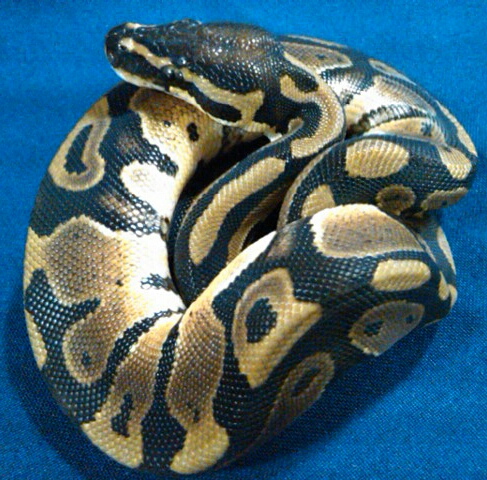
\includegraphics[width=.5\textwidth, height = 62mm]{Normal.jpg}
	\end{figure}
	\begin{figure}[H]
	\centering
	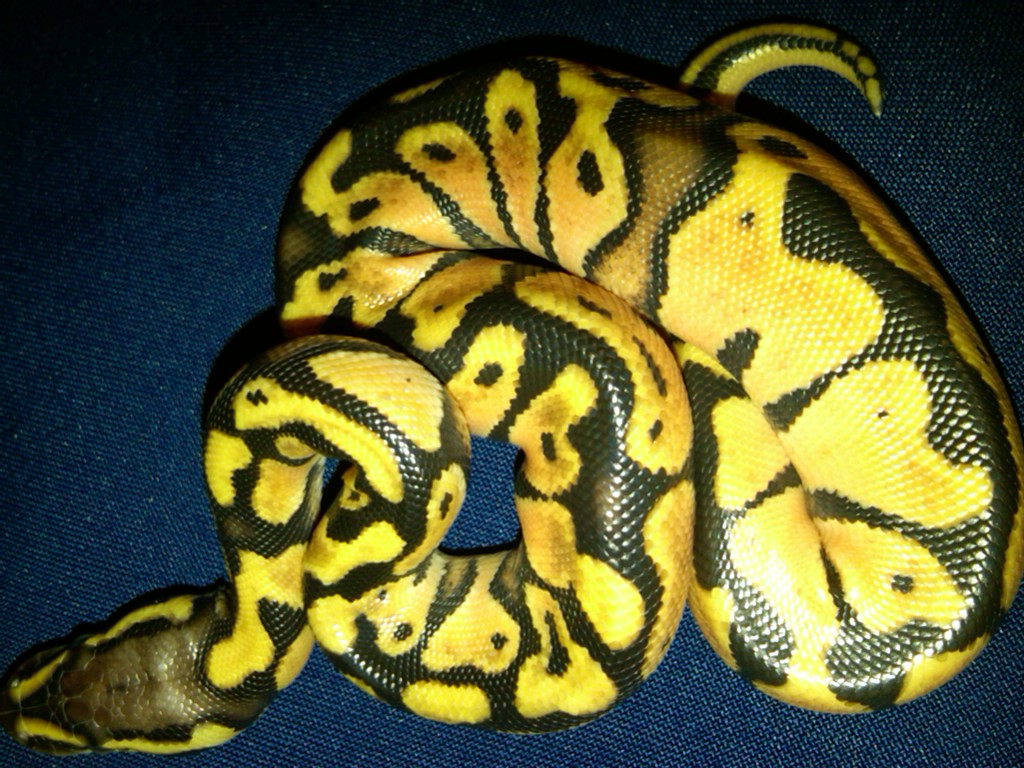
\includegraphics[width=.5\textwidth]{Pastel.jpg}
	\end{figure}
	\end{multicols}
	Note the marked difference that one trait can make in the appearance of the snake. As with dogs, certain traits are valued much higher than others. A Normal costs about \$20, whereas a Pastel costs about \$45, and Ball Pythons with another trait, called Banana, costs about \$200. As one might imagine the `cooler' looking the snake the more it will cost, so breeders seek to make more money by breeding so offspring will express more genes and therefore look `cooler'.\\
	\indent I will not go over the details of snake reproduction here, but there are certain facts that will be used in this paper and the related programs, without which the reader will undoubtedly be lost. Firstly, upon a successful (and sometimes unsuccessful) pairing of a male and female snake a set of eggs, called a clutch, is produced. Secondly, female snakes can breed up to once per breeding season, whereas a male can breed up to five times per breeding season. Lastly, a male reaches sexual maturity in about a year, whereas a female reaches sexual maturity in about two years.

	\section*{Theory}
	\indent\indent Initially, one can think of this problem as a portfolio management problem in which the Ball Python breeders are portfolio managers and the snakes are capital goods, and one can imagine that the breeders would like to maximize the present discounted value of profits from their stock of snakes. The preceding method was pioneered in  \cite{jarvis}. Comparative statics for this interpretation have been derived in the preceding paper and \cite{Paarsch}.\\\indent The previous papers assume the animals (cattle) are all homogeneous except in age and there was no improvement in breed over time, which are simply not valid assumptions in the case of snake breeding. The value of each snake in your inventory depends on the genes it expresses, which depends on what its parents were, and there is an overall improvement in your stock over time because of the selective breeding exercise, which can't be handled by the aforementioned model.\\
	\indent One could expect that after a certain point the system will settle into a steady state, and it might be a useful exercise to characterize what the steady state would look like. If the breeder's set of snakes is not homozygous (having two copies of a certain allele) for all the different genes contained in their snakes, then the system will not be in a steady state, since they will try to breed so that their snakes are homozygous for all traits since that makes them more valuable. If their whole stock of snakes is homozygous for all of the same genes except for one snake, then they will either breed the snake that's different to at least one other snake, or they will sell it. If they breed the snake that's different then there will be some snakes in stock that are not homozygous (heterozygous) for all genes, which would continue as selective breeding until all snakes were homozygous for all genes in the stock of snakes. The steady state can't occur unless all snakes have the same genes and are homozygous for them all, at which point the problem changes to be akin to the previous models. However, supposing that all snakes are homozygous for all genes except for a gene which all snakes are heterozygous for, there is some positive probability that in any finite number of periods none of the snakes will be born homozygous for that gene, so a steady state is not guaranteed to be achievable in a finite number of periods.\\
	\indent Suppose instead, that one is interested in how the system behaves before a steady state if one would even occur (as this paper is). As was shown in the previous paragraph, this would be where at least one snake is different from the others, or the snakes are all the same, but not homozygous for all traits. In this world it matters which snake you breed to which, so this becomes a matching  problem: deciding which male to breed to which females. Thinking about a single period yields the problem courtesy of \cite{becker} with a slight tweak:
	\begin{align*}
		\max_{\Pi}&\left\{ \sum_{i\in I}g\left(m_i,f_{\Pi(i)}\right) \right\}
	\end{align*}
	where $I$ is the number of male snakes, $m$ signifies a male snake, $f$ signifies a female snake, $g$ is a profit function, and $\Pi$ is a mapping from the set of males to subsets of 5 or less snakes of the set of females. In this setting the matching problem will result in neither PAM nor NAM (Positive/Negative Assortative Matching) as shown in the simple example below.\\
	\indent Suppose that one has a homozygous Fire male (\$350), a heterozygous Fire female (\$90), and a homozygous Pastel female (\$75). Suppose further that you can only breed one male to one female. The offspring of the Fire Ball Pythons paired together would have an expected value of \$220, whereas with the Fire and Pastel paired together the offspring have an expected value of \$250. This may seem to imply NAM, however if one takes the same females but replaces the male with a heterozygous Pastel (\$45), the expected value of the offspring of Pastel and Fire is \$103.75 and Pastel with Pastel has an expected value of \$60, which contradicts NAM. Now there's a serious problem, if it was PAM or NAM it would be a simple process to choose which snakes to breed to which.\\
	\indent The previous two paragraphs were about a single period decision, which is not really what a snake breeder should be doing. The snake breeder should, ideally, decide what to do this period with an eye to future time periods. Unfortunately, that turns an already difficult problem into an intractable problem, maximizing time discounted profit over an infinite time horizon, i.e.:
	\begin{align*}
		\max_{\Pi_t}&\left\{ \sum_{t=1}^{\infty}\sum_{i\in I_t}g\left(m_i,f_{\Pi_t(i)},t\right)\delta^t \right\}.
	\end{align*}
	\indent So what does one do since true optimality is intractable? The approach this paper uses is find a reasonable rule that does well, where ``well'' is defined as doing better than the rule snake breeders actually follow, and simulate in order to find the changes instilled by a change in the parameters of the system.
	\section*{Data}
	\indent I retrieved the data used for my program from the breeders at a show called Repticon in Tampa. I gathered the genetics of the snakes, the sex of the snakes, and the price of the snakes. I ran a linear regression of the traits and sex of the snake against the log of the price of the snake for snakes that had only genes represented in at least 10 snakes. This was accomplished by eliminating genes that had less than 10 snakes and eliminating the snakes with those genes in the R script \textit{modeler.R}. The resulting genes (first column) and their prices (second column) are found in \textit{newprices.csv}.
	\section*{Program}
	\indent Since most of the work in this paper has gone into developing the simulation program, \textit{snakes.py}, it seems reasonable to talk a little about what is going on in the program. The first major part of the program is that a snake is an instance of a class aptly called Snake which contains the relevant information about a snake: name, age, sex, price, traits, forebears, age it can breed, and number of times it has bred this period. The second major part of the program is the function tick which simulates what a breeder with a given decision rule will do in a year. The function tick itself calls three separate functions: breed, hypobreed, and hypobreedg.\\\indent The function breed does the following: checks whether the snakes can breed at all with regards to sex, age, and inbreeding, if they can it has a 60\% chance to generate offspring, and if it does, it generates a clutch size from the discrete triangular distribution where the minimum observable value is 3, maximum observable value is 14, and the value with the highest probability is 6, and generates that number of new snakes. The functions hypobreed and hypobreedg are used to calculate the expected revenue and expected number of genes of offspring respectively, for use with the decision rules.\\
	\indent The two decision rules that I implement are: maximize expected profit in the next time period, and maximize the expected number of genes in offspring. The first does the following:
	\begin{align*}
		\max_{\mathbf{X},\mathbf{y},\mathbf{z}}&\left\{ \sum_{i\in I}\mathbf r_i \mathbf x_i^T - 80\mathbf y^T\mathbf 1_I - 80\mathbf z^T\mathbf 1_J \right\}\\
      s.t. & \quad\mathbf X\mathbf 1_J \leq 5\mathbf 1_I \\
      &\quad \mathbf X^T \mathbf 1_I \leq \mathbf1_J\\
      &\quad \mathbf X \mathbf1_J\leq M\mathbf y\\
      & \quad\mathbf X^T\mathbf 1_I \leq M\mathbf z\\
      &\quad \mathbf y^T\mathbf 1_I + \mathbf z^T\mathbf 1_J \leq C\\
      & \quad X_{ij}, y_i, z_j \in \{0,1\}
	\end{align*}
	where:
	\begin{itemize}
	\item $I$- the set of male snakes in stock.
	\item $J$- the set of female snakes in stock.
	\item $\mathbf R$- (not shown) a matrix, the $ij$th element of which is the expected revenue of breeding male $i\in I$ and female $j\in J$.
	\item $\mathbf r_i$- the $i$th row of $\mathbf R$.
	\item $\mathbf X$- a decision matrix, the $ij$th element of which has a 1 if one should breed male $i$ with female $j$.
	\item $\mathbf x_i$- the $i$th row of $\mathbf X$.
	\item $\mathbf y$- a decision vector, the $i$th entry of which should contain 1 if one should keep male $i$.
	\item $\mathbf z$- a decision vector, the $j$th entry of which should contain 1 if one should keep female $j$.
	\item $M$- a large integer.
	\item $C$- the capacity constraint.
	\end{itemize}
	\indent Taken together the above maximizes expected profit in the next period subject to a capacity constraint and that males can breed up to 5 times per period and females up to once per period. One might also wonder why the number 80 appears in the objective, and the answer is that the average yearly cost to keep a ball python is \$80.\\
	\\\indent The second decision rule does the following:
	\begin{align*}
		\max_{\mathbf{X},\mathbf{y},\mathbf{z}}&\left\{ \sum_{i\in I}\mathbf g_i \mathbf x_i^T\right\}\\
      s.t. & \quad\mathbf X\mathbf 1_J \leq 5\mathbf 1_I \\
      &\quad \mathbf X^T \mathbf 1_I \leq \mathbf1_J\\
      &\quad \mathbf X \mathbf1_J\leq M\mathbf y\\
      & \quad\mathbf X^T\mathbf 1_I \leq M\mathbf z\\
      &\quad \mathbf y^T\mathbf 1_I + \mathbf z^T\mathbf 1_J \leq C\\
      & \quad X_{ij}, y_i, z_j \in \{0,1\}
	\end{align*}
	where the variables are the same as the last decision rule except:
	\begin{itemize}
	\item $\mathbf G$- (not shown) a matrix, the $ij$th element of which is the expected number of genes in the offspring of male $i$ and female $j$.
	\item $\mathbf g_i$- the $i$th row of $\mathbf G$.
	\end{itemize}
	\section*{Results}
	\indent Before I can make conclusions about the differences brought about by changing the parameters of the system, I need to show that my decision rule performs well. Having setup both my decision rule and a snake breeder's decision rule I ran both through 8 time periods 124 times apiece and calculated the Total Profit of each simulation with a capacity constraint of 15 snakes. The empirical cumulative distribution functions are shown on the next page.
	\begin{figure}[H]
	\centering
	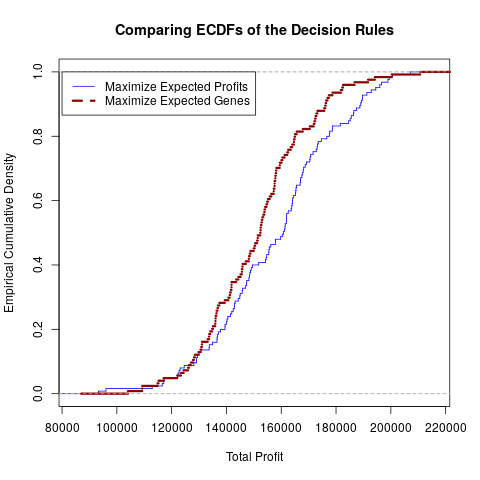
\includegraphics[width=.75\textwidth]{ECDF.png}
	\end{figure}
	The first thing to note about the above is that according to a two-sided Two-sample Kolmogorov-Smirnov test we can be 95\% (p-value .001) confident that these two ecdfs are drawn from different distributions. The second thing to note is that all risk-neutral and most risk-averse snake breeders should prefer to use my decision rule (the thinner line).\\
	\indent If one changes the snake breeder's decision rule slightly to have a naive weighting system where the most weight is placed on the best gene, second most is placed on the second best gene, and so on and so forth, the graph of the ecdfs are shown on the next page.
	\begin{figure}[H]
	\centering
	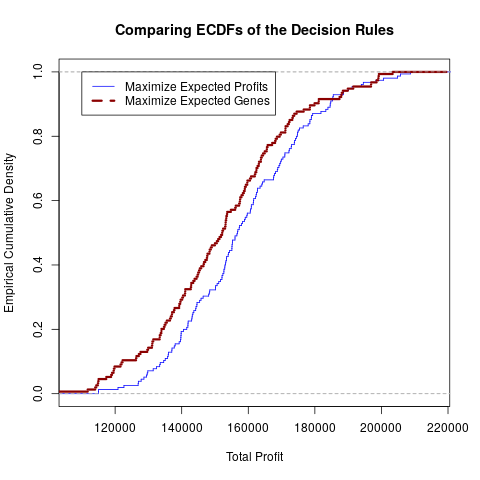
\includegraphics[width=.75\textwidth]{newECDF.png}
	\end{figure}
	
	We can be 90\% (p-value .078) confident that the two are drawn from different distributions using the same test as before. Once again all risk-neutral and most (in fact all if these distributions are close enough to the truth, since my decision rule looks like it Second Order Stochastically Dominates the snake breeder's decision rule) risk-averse snake breeders  would prefer my decision rule. One might wonder what would happen if one used a weighting system that wasn't naive, and the answer is that it would turn into maximizing expected revenue, and should do slightly worse than my decision rule.\\
	\indent Having shown that my decision rule does well, we can move on to the goal of this paper: finding how much the system changes when one alters the parameters of the system. Before we do that, let's first establish what parameters will be changed and what one might expect the result of that parameter might be.
	\subsection*{Parameters and Expectations}
		\subsubsection*{Probability of Clutch}
		\indent The current probability that a pairing will result in a clutch is .6, and since increasing that probability would increase the average number of offspring in each period it's fairly obvious to expect that the profit in each period would increase on average. Thinking a little more about it yields the following observation: there will be an effect that accumulates each period due to the fact that, since there are more snakes on average, there is a higher probability of getting better snakes each period, and since one should be choosing to keep better snakes this will have an additional positive effect on profits.
		\subsubsection*{Distribution of Clutch Size}
		There are three natural ways to modify the distribution I specified. One can change the lower bound, the highest probability, or the upper bound. Modifying one of these numbers upwards should work in a similar way to increasing the probability of a clutch, in that it will, on average, generate more snakes. This may once again have the same benefit of getting better snakes more often which will have a cumulative additional effect. On a different note, moving the lower bound up, or the upper bound down should decrease the variance of the profits.
		\subsubsection*{Male Virility}
		Since the base assumption is that a male can breed to five females, one could think of increasing that ratio as something that could be plausibly attained, and therefore something to be investigated. Since a male could still breed to five females if that would do better with regards to profit, I posit that profits could only stay the same or increase, on average, and I would place my bet on increase. Another affect that one can imagine, is that the ratio of males to females would tend to be lower, since you need fewer males to inseminate as many females, and the number of clutches can be at most the same as the number of females.
		\subsubsection*{Cost}
		As with any producer, increasing their costs should decrease their profits. This shouldn't have any strange cumulative effects until the increased cost makes the program start discarding snakes it would have otherwise kept, which shouldn't happen for small increases since most of the snakes in the initial stock are worth more than \$80.
		\subsubsection*{Capacity}
		This particular parameter is simultaneously one of the more interesting ones and the most vexing to think about. One can imagine that loosening this constraint can only have a zero or positive effect on profits, and at first blush one might guess that it would be positive. Think if you will about the following scenario: moving from a capacity of 18 to a capacity of 19. At 18 snakes it's likely that one would keep 3 males and 15 females. Suppose you have the same choices, but a capacity of 19. It's unclear whether one should use that additional space. My working hypothesis is that moving upwards will normally increase profits, but moving upwards from multiples of 6 may have no effect.
		\subsection*{Results}
		\subsubsection*{Probability of Clutch}
		\begin{figure}[H]
		\centering
		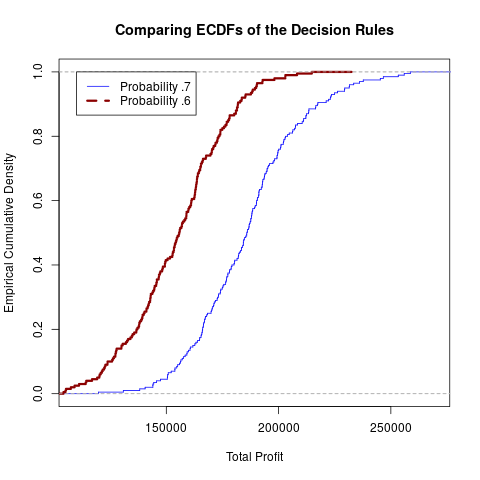
\includegraphics[width=.5\textwidth]{probECDF.png}
		\end{figure}
		As one can see from the above, it is clear that increasing the probability increases the profits, as expected. The part that requires some thought is whether or not there was the hypothesized benefit from the cumulative improvement of the genetic base. imagine with me what would happen if there wasn't a cumulative improvement. If the snakes were the same average value as they were previously, and there were just more of them than the revenue should be, on average, $16.\bar{6}\%$ higher since .7 is that percent more than .6. The costs should be roughly the same on average, which, coupled with the reasonable assumption that they should be keeping exactly 15 snakes in almost every scenario, leads me to posit that the total cost for these 8 years is $80*15*8 = 9600$. The average total profit from a probability of .6 was \$154768.6, so adding the \$9600 of cost yields an average total revenue of \$164368.6, which should increase to \$191763.4 if my hypothesis is wrong. It instead increased to \$195813. That value rejects the null hypothesis that there is no cumulative effect at an $\alpha$ of .05.
		\subsubsection*{Distribution of Clutch Size}
		\begin{figure}[H]
		\centering
		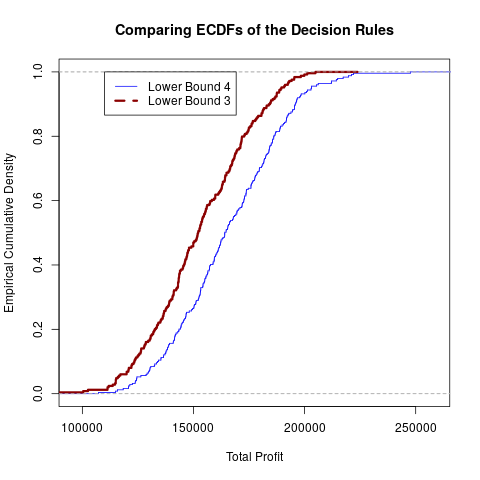
\includegraphics[width=.5\textwidth]{lbECDF.png}
		\end{figure}
		\begin{figure}[H]
		\centering
		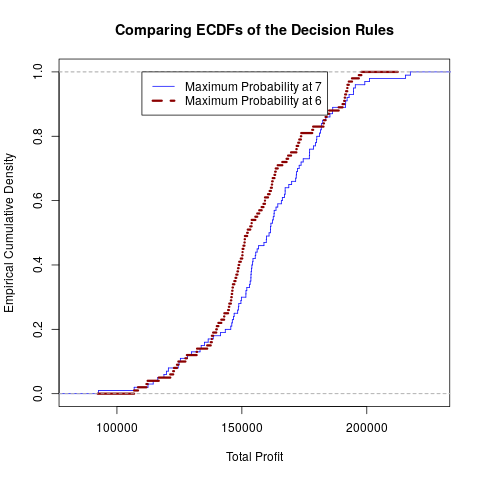
\includegraphics[width=.5\textwidth]{maxECDF.png}
		\end{figure}
		\begin{figure}[H]
		\centering
		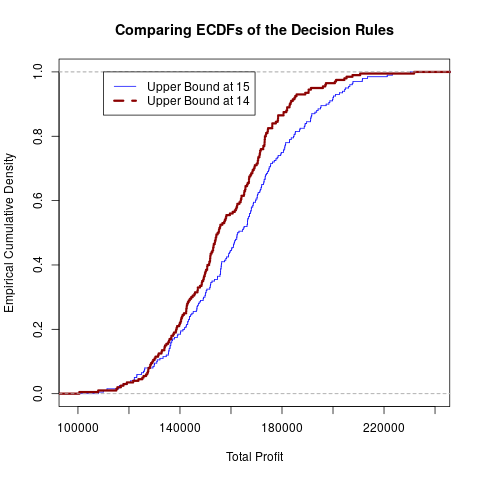
\includegraphics[width=.5\textwidth]{ubECDF.png}
		\end{figure}
		\subsubsection*{Male Virility}
		\begin{figure}[H]
		\centering
		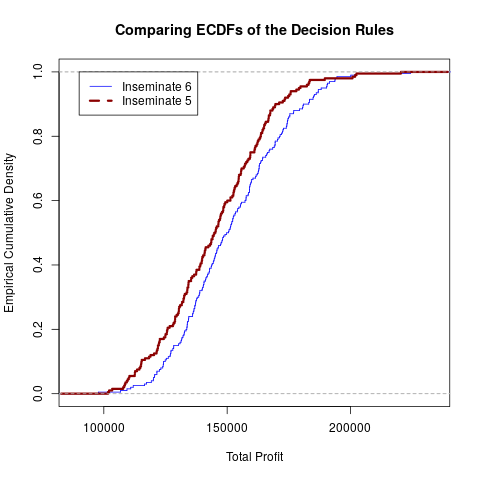
\includegraphics[width=.5\textwidth]{virECDF.png}
		\end{figure}
		\subsubsection*{Cost}
		
		\subsubsection*{Capacity}
		\begin{figure}[H]
		\centering
		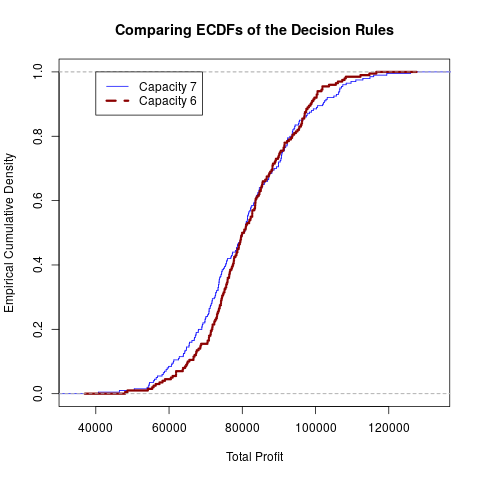
\includegraphics[width=.5\textwidth]{capECDF.png}
		\end{figure}
		\begin{figure}[H]
		\centering
		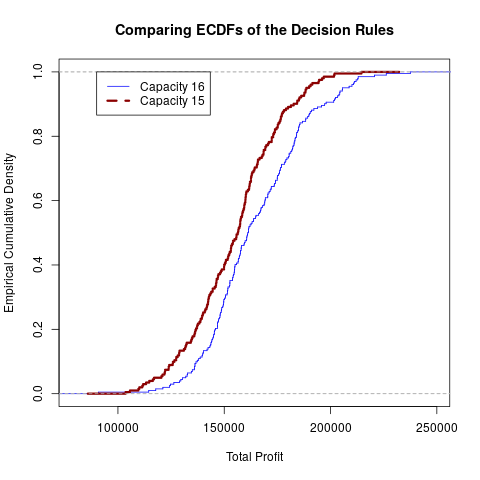
\includegraphics[width=.5\textwidth]{othcapECDF.png}
		\end{figure}
		
		
		


\bibliography{References}
\nocite{*}
\end{document}